\setcounter{footnote}{0}
\begin{frame}{Gradient Descent\footnote{Credits for this slide: Andrea Palazzi \url{https://github.com/ndrplz/deep_learning_lectures}}}
\textbf{Gradient descent} is an iterative optimization algorithm for finding the minimum of a function. How? Take step proportional to the negative of the gradient of the function at the current point.
\begin{figure}
\begin{tabular}{c}
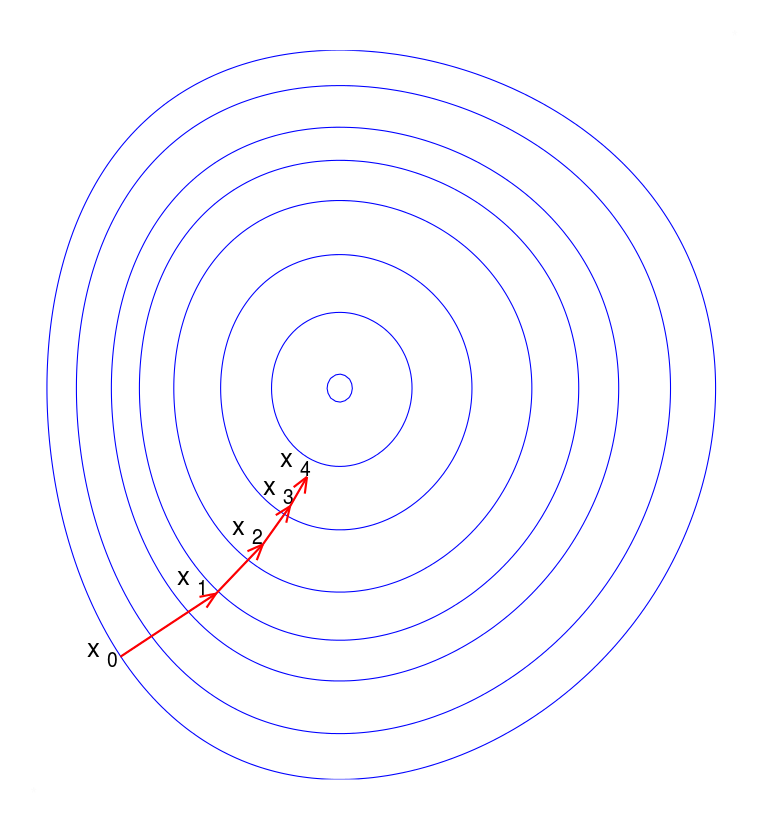
\includegraphics[width=0.2\textwidth]{img/sgd/level_sets.png}
\end{tabular}
\caption{Gradient descent on a series of level sets}
\end{figure}
\end{frame}

\setcounter{footnote}{0}
\begin{frame}{Gradient Descent Update\footnote{Credits for this slide: Andrea Palazzi \url{https://github.com/ndrplz/deep_learning_lectures}}}
If we consider a function $f(\bm{\theta})$, the \textbf{gradient descent update} can be expressed as:
\begin{equation}
\theta_j := \theta_j - \alpha \frac{\partial}{\partial \theta_j} f(\bm{\theta})
\end{equation}
for each parameter $\theta_j$.\\
\vspace{0.5cm}
The size of the step is controlled by \textbf{learning rate} $\alpha$.
\end{frame}

%%%%%%%%%%%%%%%%%%%%%%%%%%%%%%%%%%%%%%%%%%%%%%%%%%%%%%%%%%%%%%%%%%

%%%%%%%%%%%%%%%%%%%%%%%%%%%%%%%%%%%%%%%%%%%%%%%%%%%%%%%%%%%%%%%%%%
\setcounter{footnote}{0}
\begin{frame}{Visualizing Gradient Descent\footnote{Credits for this slide: Andrea Palazzi \url{https://github.com/ndrplz/deep_learning_lectures}}}
\begin{figure}
\begin{tabular}{c}
Gradient Descent for 1-d function $f(\theta)$.\\
  \animategraphics[loop,controls,width=0.9\textwidth]{1}{img/sgd/descent/descent-}{0}{7}
\end{tabular}
\end{figure}
\end{frame}


%%%%%%%%%%%%%%%%%%%%%%%%%%%%%%%%%%%%%%%%%%%%%%%%%%%%%%%%%%%%%%%%%%
\setcounter{footnote}{0}
\begin{frame}{Learning Rate\footnote{Credits for this slide: Andrea Palazzi \url{https://github.com/ndrplz/deep_learning_lectures}}}
Choosing the the right \textbf{learning rate} $\bm{\alpha}$ is essential to correctly proceed towards the minimum. A step \textit{too small} could lead to an extremely \textit{slow} convergence. If the step is \textit{too big} the optimizer could \textit{overshoot} the minimum or even \textit{diverge}. 
\begin{figure}
\begin{tabular}{ccc}
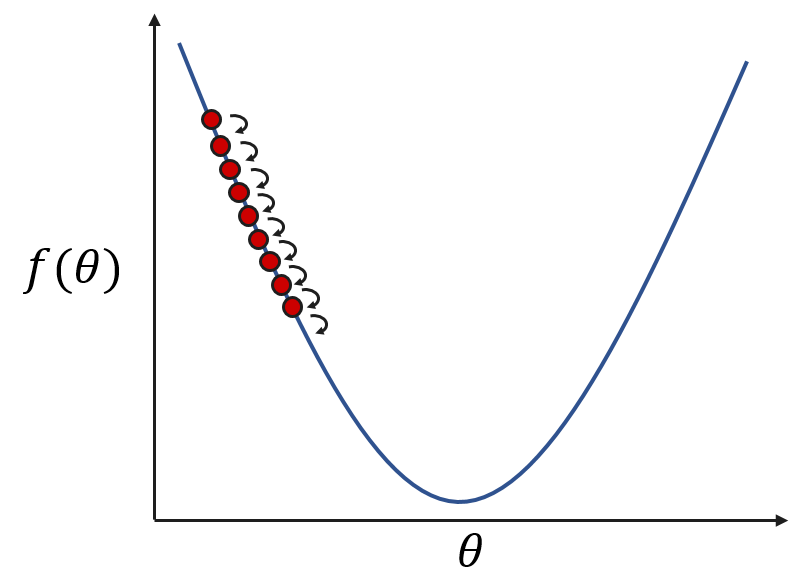
\includegraphics[width=0.35\textwidth]{img/sgd/lr_too_small.png} &
\quad &
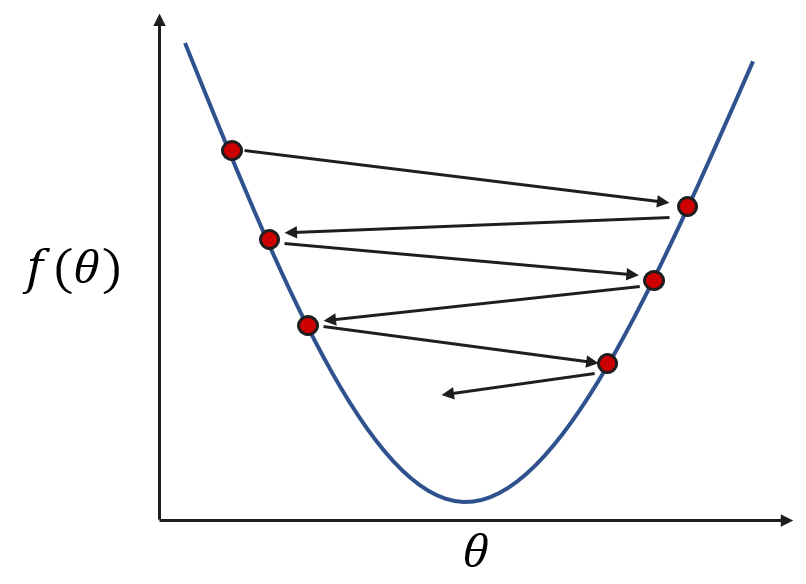
\includegraphics[width=0.35\textwidth]{img/sgd/lr_too_big.png}\\
Learning Rate too small & & Learning Rate too big
\end{tabular}
\end{figure}

\end{frame}
